
\documentclass{llncs}
\usepackage{amsmath}
\usepackage{amsfonts}
\usepackage{graphicx}
\usepackage{epstopdf}
\usepackage{subfigure}
\usepackage{floatrow}
\floatsetup[table]{capposition=top}
\newfloatcommand{capbtabbox}{table}[][\FBwidth]
\usepackage[linesnumbered,boxed]{algorithm2e}



\begin{document}
\title{Realtime Event Summarization from Tweets with Inconsistency Detection}
\author{Lingting Lin, Yunjie Wang, Chen Lin}
\institute{Department of Computer Science, Xiamen University \email{chenlin@xmu.edu.cn}}

\maketitle
\begin{abstract}
\end{abstract}
\section{Introduction}
%Motivation
Accidents, disasters, political rallies...we are eager to gather information about different kinds of live events that happen around us. In the past, we rely on experienced journalists to cover the stories. At now, thanks to the large community of micro-blogging users, we are provided with instant reports published by individuals and organizations all over the world.  More and more people today rely on microblogging contents, such as Tweets, to seek information about live events. However, the huge volume of event related tweets could be overwhelming. For example, TweeStudy shows that the majority (over $85\%$) of trending topics in microblog sphere are headline news and real-life events~\cite{kwak2010twitter}. An event summarization system is needed to facilitate knowledge management and improve user experiences.

We have witnessed rapidly increasing popularity of research efforts in event summarization from tweets~\cite{}.   Most previous work are based on extractive method, i.e. they extract a smallest set of representative tweet reports\footnote{To distinguish tweets to be summarized and tweets in the summary, we will refer the former as tweets and the latter as reports} to form a brief summary. Extractive methods are easy to implement and have shown to perform well~\cite{}. Our arguments are founded on extractive summarization methods.

%requirement: realtime
Beyond the usual requirements for text summarization systems, such as coverage and representativeness of the summary,  event summary must also be \textbf{realtime}. On one hand, the response must be fast. The summary must be efficiently updated as new tweets arrive. On the other hand, the summary must report the current status of the event. As an ongoing event often involves changing information, report must be updated to include new information when it emerges.

%inconsistency
During the update process, the integrity of the summary must be preserved.  An outdated report must be replaced if it leads to \textbf{inconsistency} in the summary. An inconsistent summary is harmful for most live events because it is confusing and misleading. In particular, for natural disaster or group incidents,  users are interested on  information such as number of injuries, suspects description and so on. We here list three scenarios when a former report needs to be replaced because of inconsistency. (1) The information changes as a natural consequence of event evolution. For example, in an earthquake the number of injuries is increasing over time. Thus the numbers in previous summaries become obsolete and they should be replaced by the most up-to-date numbers. (2) Multiple information sources provide conflicting information. For example, the number of injuries is often estimated by several parties, such as  bystanders, hospitals and so on. When a more authoritative source, such as the local government announces the new estimate, the old estimates in previous summaries are no longer credible and must be replaced. (3) The information in previous summaries is wrong. For example, the police have suspected the wrong person and now they update the description. In this case, the realtime event summarization system must select the correct tweet to replace former reports.


%open problem: no related work prevent inconsistency in
Realtime event summarization from Tweets is still an open problem. In the literature, most of previous works treat the problem as producing different forms of summaries from a static set of tweets~\cite{}. A few recent research works focused on efficient algorithms to summarize the tweet streams~\cite{}. Their summarization systems are based on coarse grained semantic analysis, and thus are not able to detect inconsistency. Though we have shown that integrity of the event summary is crucial, to the best of our knowledge, none of the previous works is able to produce a realtime event summarization which is guaranteed to exclude inconsistent information.


%challenge
Two challenges arise in producing realtime event summarization without inconsistent information.

%Algorithm
The first challenge lies in the macro-level algorithm. Realtime summarization requires an efficient algorithm to analyze the streaming tweets. As the amount of available tweets constantly increases to infinity, re-computation based on a complete set of all tweets up to the current timestamp is infeasible. The ideal algorithm is to  incorporate new tweets as they become available, and discard old tweets when possible to limit the storage and speed up processing.

%inconsistency detection
The second challenge is related to the micro-level analysis to detect inconsistency. Inconsistency detection is based on pair-wise similarity. Coarse grained semantic analysis, such as the cosine similarity measure based on the bag of words representation in previous works~\cite{} is suitable to capture topic similarity in a summarization, but is not able to detect inconsistent information. Inconsistency is revealed via word order and syntactic structures. We need to assess information similarity based on the combination of semantic, lexical and syntactic analysis. Furthermore, inconsistency detection is computationally expensive. It is important to avoid unnecessary pair-wise comparisons.

%idea: micro level:
Our goal in this paper is to design a system that delivers realtime summary with integrity from tweets. To address the first challenge, we assume that, the realtime summarization problem given a small batch of new tweets can be modeled as two integer programming problems, one of which on the old tweets, and another on the new batch. Both integer programming problems can be relaxed to linear programming problems and be solved by the simplex method. In each update we first optimize the problem on the new batch. We use the solution on the new batch to modify the problem on the old tweets and incrementally update the summary.  In this manner, we do not need to store or operate on the complete tweet set and the full similarity matrix.


To address the second challenge, we propose skeleton similarity: a new similarity metric to assess information similarity between any pair of tweets. An inconsistency detection strategy, which is a combination of the skeleton similarity and authority estimation heuristics, is then adopted in the pivoting operation in the simplex method. It has two advantages in embedding the skeleton similarity computation in the simplex algorithm. (1) It significantly reduces the number of information similarity comparisons. (2) It ensures that the former summary will be replaced by most up-to-date, authoritative and correct information.


%contributions
Our contributions are three folds. (1) The integrity of event summary is a relatively unexplored area in Tweet summarization. We propose to improve the integrity of event summarization by explicit inconsistency detection. (2) Our system is targeted towards text streams. We differ from existing work in that we enable incremental update in the simplex method framework. (3) We propose a novel skeleton similarity to efficiently and effectively capture inconsistency.

%paper structure
This paper is organized as follows. We briefly survey the related work in Sec.~\ref{sec:related}. In Sec.~\ref{sec:static}, we first introduce the idea of modeling a summarization problem as an integer programming problem and the standard simplex procedure to solve the relaxed linear programming problem. In Sec.~\ref{sec:dynamic}, we give the problem definition for realtime event summarization given a small batch of new tweets and the modified simplex solution. In Sec.~\ref{sec:inconsistency}, we describe the inconsistency detection strategy. We present and analyze the experimental results on a real data set in Sec.~\ref{sec:experiment}. We conclude our work and suggest future directions in Sec.~\ref{sec:conclusion}.

\section{Related Work}\label{sec:related}
%tweet summarization

%Event summarization


\section{Static Summarization}\label{sec:static}
In this section, we first model the (standard) static summarization problem as an integer programming problem. We then introduce background knowledge about the simplex method. We finally give a outline for the algorithm to solve static summarization.
\subsection{Problem Definition}
Suppose that we have a universe of $N$ tweets, within which $M$ tweets are credible and relevant. The extractive method for any static summarization is to select a few representative reports from the tweet universe to form the summary. To model this problem, we use a vector $\tilde{\mathbf{x}}\in R^N$ , where each element $\tilde{\mathbf{x}}_j\in \{0,1\}$ is a binary variable. If a tweet $i$ is chosen to be a report in the summary, the corresponding $\tilde{\mathbf{x}}_i=1$ . Otherwise, we set  $\tilde{\mathbf{x}}_i=0$. We use another $N$-dim vector $\tilde{\mathbf{c}}\in R^M$ to describe the loss of choosing each tweet as a report. $\tilde{\mathbf{A}}\in R^{M\times N}$  is a similarity matrix, where $\tilde{a}_{i,j}$  is the similarity between a credible and relevant tweet $i$ and a candidate tweet $j$ in the tweet universe. $\mathbf{b}\in R^{M}$ is a weight vector, where $b_{i}>0$ indicates the importance of $i$ being covered in the summary. Our objective is

\begin{equation}\label{equ:integerstatic}
\min \tilde{\mathbf{c}}^T\tilde{\mathbf{x}}\textrm{ subject to } \tilde{\mathbf{A}}\tilde{\mathbf{x}}\geq \mathbf{b}, \tilde{\mathbf{x}}\in \{0,1\}.
\end{equation}

\subsection{The Simplex Method}
We transform the integer programming problem in Equ.~\ref{equ:integerstatic} to a bounded linear programming problem by making the following adjustments: $\mathbf{c}=[\tilde{\mathbf{c}},\mathbf{0}],\mathbf{x}=[\tilde{\mathbf{x}},\mathbf{z}]^T,\mathbf{A}=[\tilde{\mathbf{A}},-\mathbf{I}]$, where $\mathbf{I}$ is the $M\times M$ identity matrix. Therefore we have the following objective

\begin{equation}\label{equ:linear}
\min \mathbf{cx} \textrm{ subject to } \mathbf{Ax} = \mathbf{b}, \mathbf{x}\geq \mathbf{0},\tilde{\mathbf{x}} \leq \mathbf{1}.
\end{equation}

The linear programming problem in Equ.~\ref{equ:linear} can be solved by the simplex method. Each iterate in the simplex method is a basic feasible point that (1) it satisfies $\mathbf{Ax} = \mathbf{b}, \mathbf{x}\geq \mathbf{0},\tilde{\mathbf{x}} \leq \mathbf{1}$ and (2) there exists three subsett $\mathcal{B,U.L}$ of the index set $\mathcal{A}=\{1,2,\cdots N\}$ such that $\mathcal{B}$ contains exactly $M$ indices, $\mathcal{A}=\mathcal{B}\cup \mathcal{U} \cup \mathcal{L}$ and $i \in \mathcal{U} \Rightarrow x_i=1,i \in \mathcal{L} \Rightarrow x_i=0$.

The major issue at each simplex iteration is to decide which index to be removed from the basis $\mathcal{B}$ and replaced by another index outside the basis $\mathcal{B}$.  As the optimal is achieved when the KKT conditions are satisfied, in each simplex iteration first  a pricing step is conducted to check on the KKT conditions.  Let's compute $\mathbf{y} = {\mathbf{B}^T}^{-1}\mathbf{c_B}$, $\bar{c_j} = c_j - y^T\mathbf{A}_{,j}^{'}$. If $x_j = 0, \bar{c_j} > 0$ and $x_j = 1,\bar{c_j} < 0$,  the KKT conditions are satisfied and the problem is solved. Otherwise a pivoting operation is implemented to select entering and leaving indices.

We should keep in mind that the simplex iterations are run on basic feasible points. To obtain an easy start of basic feasible points, we solve the following linear programming problem.

\begin{equation}\label{equ:linearphaseI}
\min \mathbf{e^{T}s} \textrm{ subject to } \mathbf{Ax} + \mathbf{Is} = \mathbf{b}, \mathbf{x}\geq \mathbf{0},\tilde{\mathbf{x}} \leq \mathbf{1},\mathbf{s}\geq \mathbf{0},
\end{equation}

where $\mathbf{e}$ is the vector of all ones, $\mathbf{I}$ is a diagonal matrix whose diagonal elements are $I_{ij}=1$. $\mathbf{s}$ are called artificial variables. It is easy to see that the solution to Equ.~\ref{equ:linearphaseI} is a basic feasible point for Equ.~\ref{equ:linear}, if the objective $\mathbf{e^{T}s}=0 $.

The remaining problem is that the solution we obtained for Equ.~\ref{equ:linear} are not integers. We therefore present to round the solutions by

\begin{equation}
p(x_i=1)= x_i
\end{equation}

%delete?
We sort the solution we obtained for Equ.~\ref{equ:linear} in descending order of values and find the minimum tweets to cover all credible and relevant tweets.And then delete inconsistent information in summarys by inconsistency detection. Delete the lower weight tweet,if they have equal weight then delete the earlier one.

To conclude this section, we present Algorithm.~\ref{alg:framework}

\begin{algorithm}\label{alg:framework}
\caption{The pseudo code of the framework for static summarization}
\KwIn{$\mathbf{\tilde{c},b, \tilde{A}}$}
\KwOut{$\mathbf{x}$}

Initialize $\mathbf{x}=\mathbf{0},\mathbf{s}=\mathbf{b}$\;
Solve $\min \mathbf{e^{T}s} \textrm{ subject to } \mathbf{Ax} + \mathbf{Is} = \mathbf{b}, \mathbf{x}\geq \mathbf{0},\tilde{\mathbf{x}} \leq \mathbf{1},\mathbf{s}\geq \mathbf{0}$ by simplex method\;
Keep $\mathbf{x}$, set $\mathbf{c}=[\tilde{\mathbf{c}},\mathbf{0}],\mathbf{x}=[\tilde{\mathbf{x}},\mathbf{z}]^T,\mathbf{A}=[\tilde{\mathbf{A}},-\mathbf{I}]$ \;
Solve $\min \mathbf{cx} \textrm{ subject to } \mathbf{Ax} = \mathbf{b}, \mathbf{x}\geq \mathbf{0},\tilde{\mathbf{x}} \leq \mathbf{1}$ by simplex method\;
Rounding $\mathbf{x}$\;
%delete?
\end{algorithm}



\section{Dynamic Summarization}\label{sec:dynamic}

\subsection{Problem Definition}
%first show that we don't need A by proving the constraint 1 hold by itself for all scenarios (conflicting, outdate, better converage)
\begin{equation}
\min c_0x_0+c_1x_1\\
s.t. \begin{bmatrix}
A & D \\
D^T & B
\end{bmatrix}\begin{bmatrix}
 x_0\\
x_1
\end{bmatrix}\geq \begin{bmatrix}
b_0\\
b_1
\end{bmatrix}
\end{equation}

%check whether constraint 2 is satisfied, note that D is small due to the sparseness of x_0
$D^Tx_0\geq b_1$

%if b_1 largely not covered, outdated, change constraint


%else implement simplex

%if an index gets out, check if its conflicting by measuring structural similarity
\subsection{Online Simplex Method}
\begin{algorithm}
\caption{the bounded simplex method}
\KwIn{$\mathbf{c}=[\mathbf{e},\mathbf{0}], \mathbf{x}^{'} = [\mathbf{x},\mathbf{s}]^T$ and $\mathbf{A}^{'} = [\mathbf{A},\mathbf{I}]$}
\KwOut{$\mathbf{x_B^{'}} = \mathbf{A_B^{'}}^{-1}(\mathbf{b} - \mathbf{u})$, where $\mathbf{u} = \Sigma_{j\in U} \mathbf{A}_{,j}^{'}$}

%$\mathbf{B} \leftarrow$ \{the indices of the artificial variables\}\;
%$\mathbf{x_N}$ = 0\;
Pricing $\mathbf{y} = {\mathbf{B}^T}^{-1}\mathbf{e_B}$\;
Compute $\bar{c_j} = c_j - y^T\mathbf{A}_{,j}^{'}$\;
\While{$\exists x_j = 0, \bar{c_j} < 0$ or $x_j = 1,\bar{c_j} < 0$}
{
    $q = \arg\max_{j} \left\{\bar{c_j} \forall j\in\{\mathbf{z_N}, \mathbf{s_N}, \mathbf{x_L}  \},-\bar{c_j} \forall j\in\mathbf{x_U}  \right\}$\;
    $d = \mathbf{B}^{-1}\mathbf{A}_{,q}^{'}$\;
    \If{$q \in \{ \mathbf{z_N}, \mathbf{s_N}\}$}
    {
        $x_q^{new} = \min_i \left\{\{\frac{x_{\mathbf{B}_{i}}}{d_i}, \frac{s_{\mathbf{B}_{i}}}{d_i}, \frac{z_{\mathbf{B}_{i}}}{d_i}\} \forall d_i>0,\{\frac{x_{\mathbf{B}_{i}}-1}{d_i}\} \forall d_i<0\right\}$\;
        $\mathbf{x}_{\mathbf{B}^{old}}^{'new} = \mathbf{x}_{\mathbf{B}^{old}}^{'old} - dx_q^{new}$\;
        $p=\arg\min_{i}$\;
        $\mathbf{B}^{new} \leftarrow \mathbf{B}^{old} - \{p\} \bigcup \{q\}$\;
    }
    \If{$q \in L$}
    {
        $x_q^{new} = \min_i \left\{\{\frac{x_{\mathbf{B}_{i}}}{d_i}, \frac{s_{\mathbf{B}_{i}}}{d_i}, \frac{z_{\mathbf{B}_{i}}}{d_i}\} \forall d_i>0, \{\frac{x_{\mathbf{B}_{i}}-1}{d_i}\} \forall d_i<0, 1 \right\}$\;
        $\mathbf{x}_{\mathbf{B}^{old}}^{'new} = \mathbf{x}_{\mathbf{B}^{old}}^{'old} - dx_q^{new}$\; \If{$x_q^{new} \neq 1$}
        {
            $p=\arg\min_{i}$\;
            $\mathbf{B}^{new} \leftarrow \mathbf{B}^{old} - \{p\} \bigcup \{q\}$\;
        }
    }
    \If{$q \in U$}
    {
        $x_q^{new} = 1 - \min_i \left\{\{\frac{x_{\mathbf{B}_{i}}}{-d_i}, \frac{s_{\mathbf{B}_{i}}}{-d_i}, \frac{z_{\mathbf{B}_{i}}}{-d_i}\} \forall d_i<0, \{\frac{1-x_{\mathbf{B}_{i}}}{d_i}\} \forall d_i>0, 1 \right\}$\;
        $\mathbf{x}_{\mathbf{B}^{old}}^{'new} = \mathbf{x}_{\mathbf{B}^{old}}^{'old} + d(1-x_q^{new})$\;
        \If{$x_q^{new} \neq 0$}
        {
            $p=\arg\min_{i}$\;
            $\mathbf{B}^{new} \leftarrow \mathbf{B}^{old} - \{p\} \bigcup \{q\}$\;
        }
    }
}

\end{algorithm}



\section{Inconsistency Detection}\label{sec:inconsistency}

\section{Experiment}\label{sec:experiment}
\subsection{Experimental Setup}
%Data set
We use the twitter event data set~\cite{}. The corpus includes data for 30 different Twitter datasets associated with real world events. The datasets were collected between 2012 and 2016, always using the streaming API with a set of keywords. Different types of tweets are presented, including repliesand retweets. The corpus is multilingual, including English, Japanese and so on. For the purpose of event summarization, we select 10 events and filter relevant tweets by only select tweets in English. More details of the data set are illustrated in Table ~\ref{table:static}.

\begin{table}[htp]\label{table:static}
\caption{Statistics of the data set}
\begin{center}
\begin{tabular}{|c|c|c|c|c|c|}
    \hline
    Event & Number of tweets & Time period & Average Length of tweets &  Number of terms\\
    \hline
    EOutbreak & 12983 & 2014/7/1 $\sim$ 2014/7/31 & 93 & 15 \\
    \hline
    GUattack & 21000 & 2014/6/2 $\sim$ 2014/7/17 & 103 & 15 \\
    \hline
    HProtest & 27000 & 2014/9/26 $\sim$ 2014/10/17 & 96 & 14 \\
    \hline
    THagupit & 10315 & 2014/12/5 $\sim$ 2014/12/11 & 92 & 14 \\
    \hline
    CHShoot & 15000 & 2015/1/7 & 95 & 15 \\
    \hline
    HPatricia & 9288 & 2015/10/24 $\sim$ 2015/12/8 & 88 & 13 \\
    \hline
    RWelcome & 19725 & 2015/9/2 $\sim$ 2015/11/24 & 103 & 15 \\
    \hline
    BAExplossion & 15000 & 2016/3/22 & 91 & 14 \\
    \hline
    HPCyprus & 14917 & 2016/3/29 $\sim$ 2016/3/30 & 92 & 15\\
    \hline
    LBlast & 13423 & 2016/3/27 $\sim$ 2016/3/30 & 95 & 15\\
    \hline
\end{tabular}
\end{center}
\label{default}
\end{table}

%Preprocessing
In pre-processing corpus, we use the Bloom Filter algorithm to filter duplicate tweets. Emoji expressions,http links and mentions (@somebody)are removed from the vocabulary.


%Ground truth
Ground truth For the 10 events in corpus,2 students are invited to manually extract tweets to form the summarization for each event.

%comparative methods
The comparative methods are  state-of-the-art summarization methods.

(1)LPR

(2)MSSF

(3)SNMF

(4)Sumblr


%Operating system
We implemented all algorithms in java and all experiments have been executed on a server with an AMD Opteron Processor 280 2.40G Hz (4 cores)and main memory 8G bytes.

\subsection{Summarization Performance}
%goal

%evaluation
The measurement is mainly based on Recall-Oriented Understudy for Gisting Evaluation(ROUGE) an evaluation toolkit for document summarization[23] which automatically determines the quality of a summary by comparing it with the human generated summaries through counting the number of their overlapping textual units (e.g., n-gram, word sequences, and etc.). In particular, F-measure scores of 8 evaluations are presented for our experiments.


%results figure
\begin{figure}
    \centering
    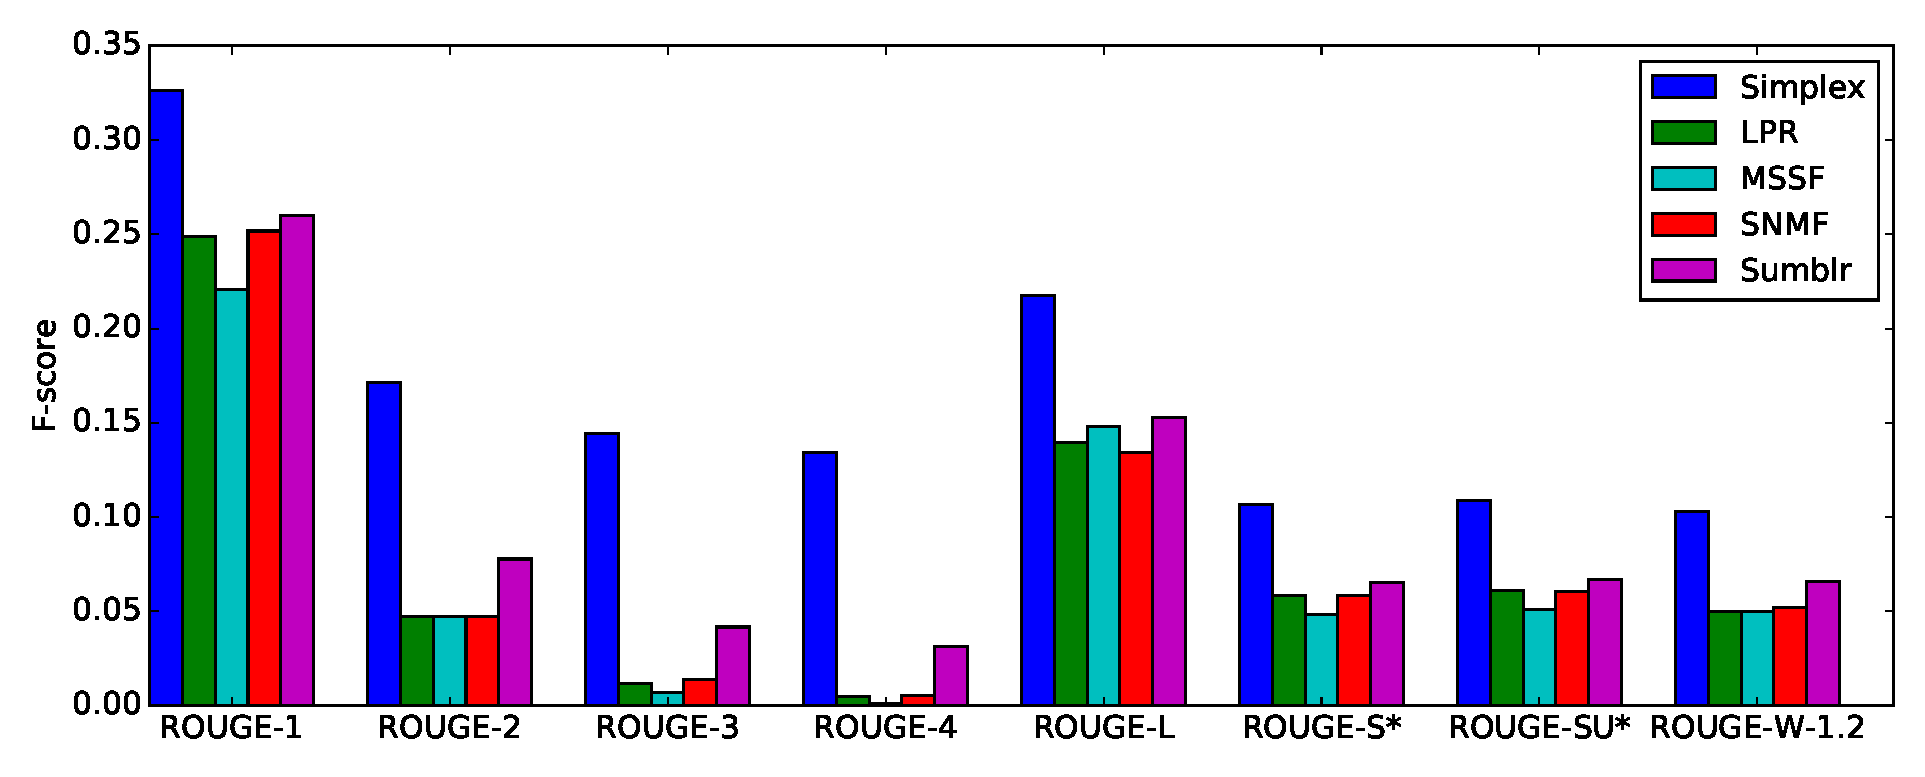
\includegraphics[scale=0.6]{rouge.eps}

\end{figure}

\begin{table}[htp]\label{table:update 0f simplex}
\caption{the updateRatio of Simplex}
\begin{center}
\begin{tabular}{|c|c|c|c|}
    \hline
    Event & Time1 & Time2 & Time3 \\
    \hline
    EOutbreak & 0 & 0.57 & 0.38 \\
    \hline
    GUattack & 0 & 0.36 & 0.33 \\
    \hline
    HProtest & 0.38 & 0.67 & 0.96 \\
    \hline
    THagupit & 0 & 0.1 & 0.62\\
    \hline
    CHShoot & 0.94 & 0.62 & 0.25\\
    \hline
    HPatricia & 0 & 0.75 & 0.83\\
    \hline
    RWelcome & 0.20 & 0.50 & 0\\
    \hline
    BAExplossion & 1 & 0.67 & 0.80\\
    \hline
    HPCyprus & 0.88 & 0.65 & 0.76\\
    \hline
    LBlast & 0.22 & 0.50 & 0.69\\
    \hline
\end{tabular}
\end{center}
\label{default}
\end{table}

\begin{table}[htp]\label{table:update 0f sumblr}
\caption{the updateRatio of Sumblr}
\begin{center}
\begin{tabular}{|c|c|c|c|}
    \hline
    Event & Time1 & Time2 & Time3 \\
    \hline
    EOutbreak & 0.75 & 0.30 & 0.20 \\
    \hline
    GUattack & 0.65 & 0.50 & 0.30 \\
    \hline
    HProtest & 0.35 & 0.40 & 0.30 \\
    \hline
    THagupit & 0.65 & 0.45 & 0.10\\
    \hline
    CHShoot & 0.20 & 0.05 & 0.10\\
    \hline
    HPatricia & 0.25 & 0.20 & 0\\
    \hline
    RWelcome & 0.35 & 0.35 & 0.20\\
    \hline
    BAExplossion & 0.45 & 0.35 & 0\\
    \hline
    HPCyprus & 0.30 & 0.15 & 0.25\\
    \hline
    LBlast & 0.30 & 0.25 & 0.05\\
    \hline
\end{tabular}
\end{center}
\label{default}
\end{table}

\begin{table}[htp]\label{table:update 0f mssf}
\caption{the updateRatio of MSSF}
\begin{center}
    \begin{tabular}{|c|c|c|c|}
    \hline
    Event & Time1 & Time2 & Time3 \\
    \hline
    EOutbreak & 0.41 & 0.29 & 0.24 \\
    \hline
    GUattack & 0.62 & 0.18 & 0.18 \\
    \hline
    HProtest & 0.65 & 0.22 & 0.17 \\
    \hline
    THagupit & 0.39 & 0.61 & 0.18\\
    \hline
    CHShoot & 0.33 & 0.39 & 0.18\\
    \hline
    HPatricia & 0.47 & 0.29 & 0\\
    \hline
    RWelcome & 0.44 & 0.62 & 0.17\\
    \hline
    BAExplossion & 0.39 & 0.12 & 0.12\\
    \hline
    HPCyprus & 0.11 & 0.17 & 0.17\\
    \hline
    LBlast & 0.35 & 0.50 & 0.33\\
    \hline
    \end{tabular}
\end{center}
\label{default}
\end{table}

\subsection{Inconsistency Detection Performance}
%comparative methods
In addition of the state-of-the-art summarization methods, for comparison on inconsistency detection, we adopted some naive methods

%result table or figure
\begin{table*}
\begin{floatrow}
\capbtabbox{
    \begin{tabular}{|c|c|c|c|c|}
    \hline
    Event & Time0 & Time1 & Time2 & Time3 \\
    \hline
    EOutbreak & 0.65 & 0.70 & 0.65 & 0.70 \\
    \hline
    GUattack & 0.60 & 0.55 & 0.40 & 0.50 \\
    \hline
    HProtest & 0.60 & 0.55 & 0.55 & 0.50 \\
    \hline
    THagupit & 0.70 & 0.75 & 0.70 & 0.65\\
    \hline
    CHShoot & 0.85 & 0.70 & 0.75 & 0.70\\
    \hline
    HPatricia & 0.75 & 0.75 & 0.75 & 0.75\\
    \hline
    RWelcome & 0.65 & 0.60 & 0.65 & 0.65\\
    \hline
    BAExplossion & 0.80 & 0.60 & 0.60 & 0.55\\
    \hline
    HPCyprus & 0.50 & 0.55 & 0.55 & 0.55\\
    \hline
    LBlast & 0.65 & 0.60 & 0.55 & 0.55\\
    \hline
    \end{tabular}
    }{
    \caption{the inconsistency of Sumblr}
    \label{table:inconsistency 0f Sumblr}
}

\capbtabbox{
    \begin{tabular}{|c|c|c|c|c|}
    \hline
    Event & Time0 & Time1 & Time2 & Time3 \\
    \hline
    EOutbreak & 0.76 & 0.71 & 0.76 & 0.78 \\
    \hline
    GUattack & 0.62 & 0.59 & 0.59 & 0.47 \\
    \hline
    HProtest & 0.27 & 0.33 & 0.44 & 0.44 \\
    \hline
    THagupit & 0.83 & 0.83 & 0.82 & 0.82\\
    \hline
    CHShoot & 0.83 & 0.78 & 0.76 & 0.71\\
    \hline
    HPatricia & 0.71 & 0.71 & 0.76 & 0.76\\
    \hline
    RWelcome & 0.69 & 0.75 & 0.72 & 0.72\\
    \hline
    BAExplossion & 0.67 & 0.71 & 0.76 & 0.83\\
    \hline
    HPCyprus & 0.83 & 0.89 & 0.72 & 0.65\\
    \hline
    LBlast & 0.41 & 0.56 & 0.50 & 0.56\\
    \hline
    \end{tabular}
    }{
    \caption{the inconsistency of MSSF}
    \label{table:inconsistency 0f MSSF}
}
\end{floatrow}
\end{table*}

\begin{table}[htp]\label{table:inconsistency 0f others}
\caption{the inconsistency of others}
\begin{center}
\begin{tabular}{|c|c|c|}
    \hline
    Event & SNMF & LPR \\
    \hline
    EOutbreak & 0.67 & 0.80 \\
    \hline
    GUattack & 0.47 & 0.40 \\
    \hline
    HProtest & 0.20 & 0.10 \\
    \hline
    THagupit & 0.33 & 0.20\\
    \hline
    CHShoot & 0.60 & 0.60\\
    \hline
    HPatricia & 0.53 & 0.50\\
    \hline
    RWelcome & 0.33 & 0.20\\
    \hline
    BAExplossion & 0.33 & 0.30\\
    \hline
    HPCyprus & 0.33 & 0.30\\
    \hline
    LBlast & 0.07 & 0.10\\
    \hline
\end{tabular}
\end{center}
\label{default}
\end{table}

\subsection{Efficiency Study}

%goal

%result figure

\begin{figure}
    \centering
    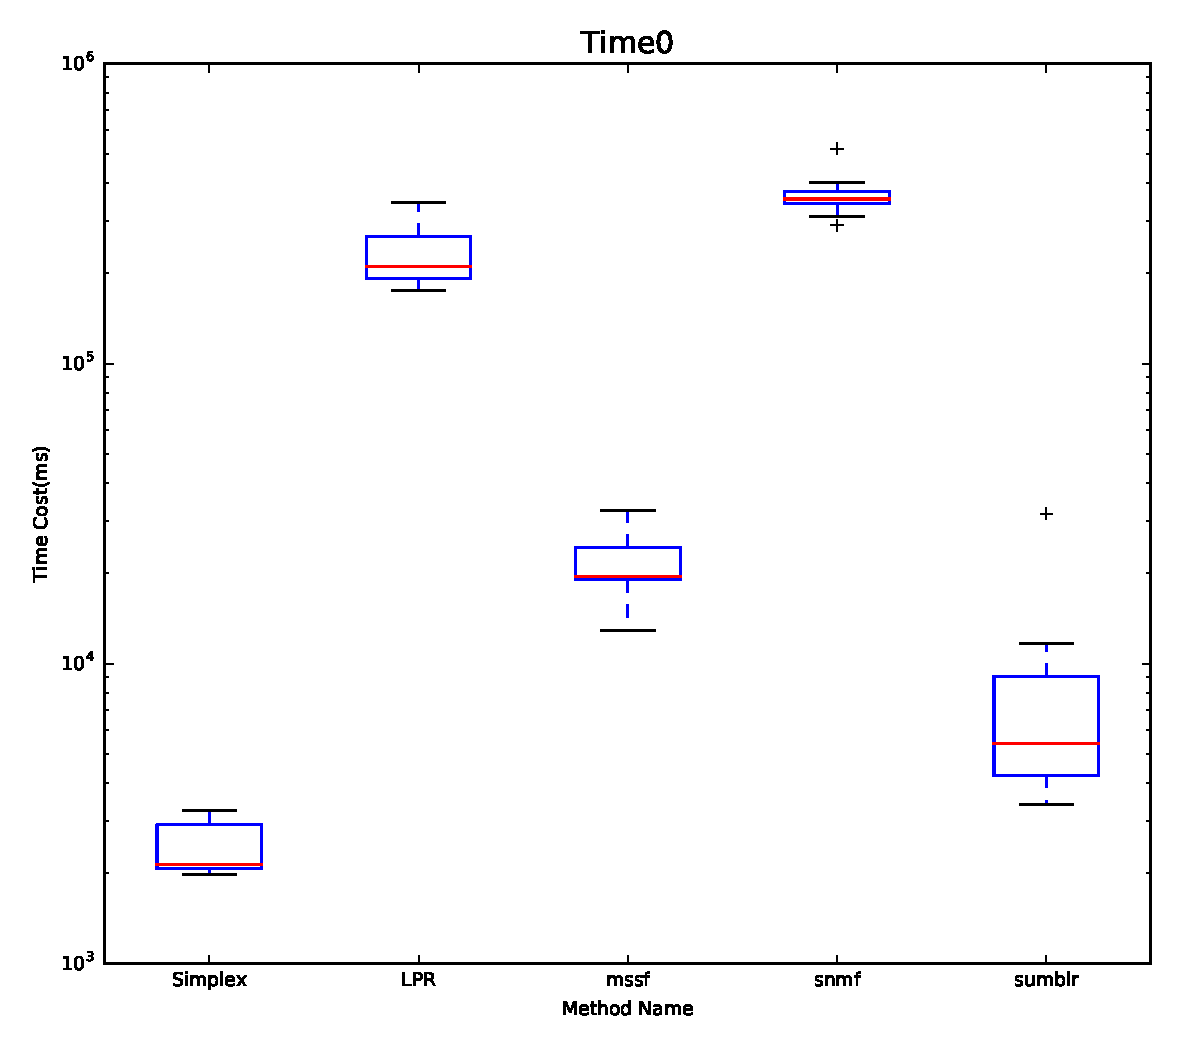
\includegraphics[scale=0.5]{log_time0.eps}

    \label{fig:side:a}
\end{figure}

\begin{figure}
    \centering
    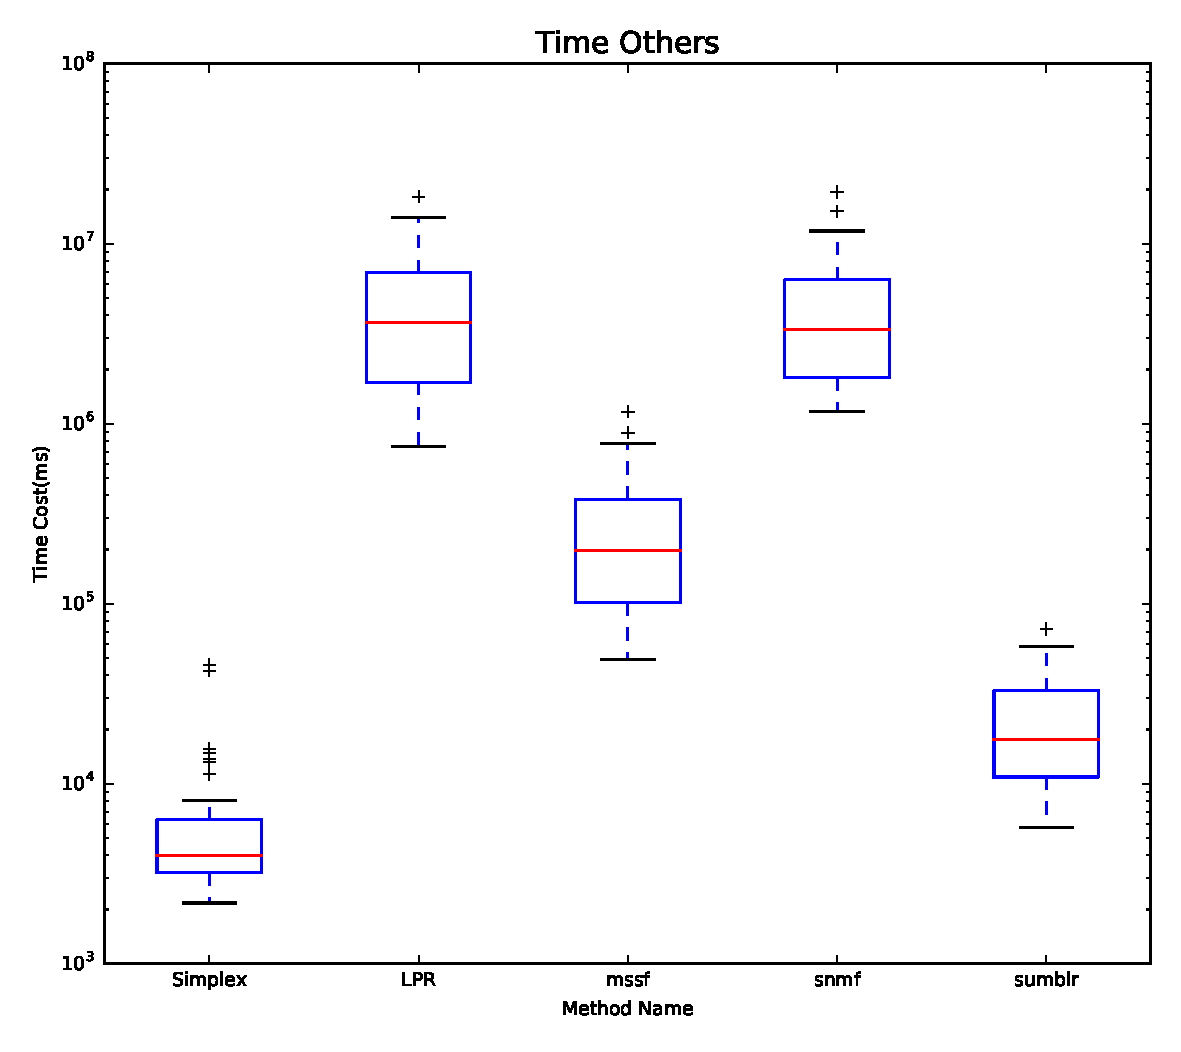
\includegraphics[scale=0.5]{log_time1.eps}
    \caption{fig2}
    \label{fig:side:b}
\end{figure}

\subsection{Effects of Parameters}

%goal

%result figure
\begin{figure}
    \centering
    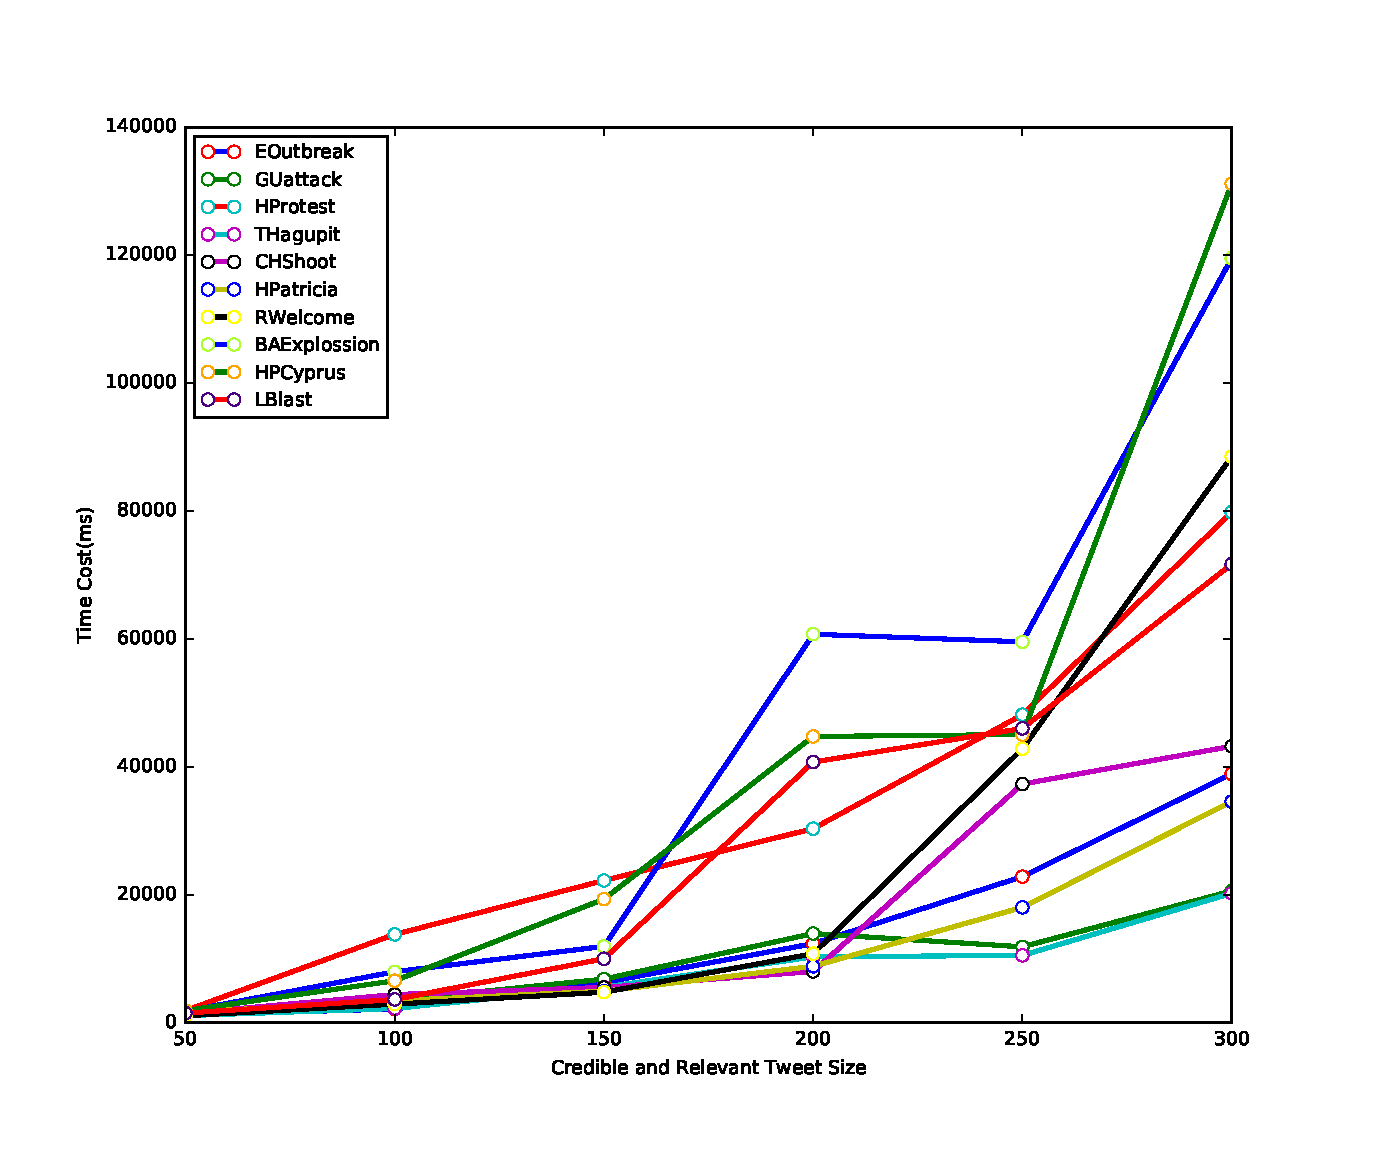
\includegraphics[scale=0.5]{summary-timecost.eps}

\end{figure}

\begin{figure}
    \centering
    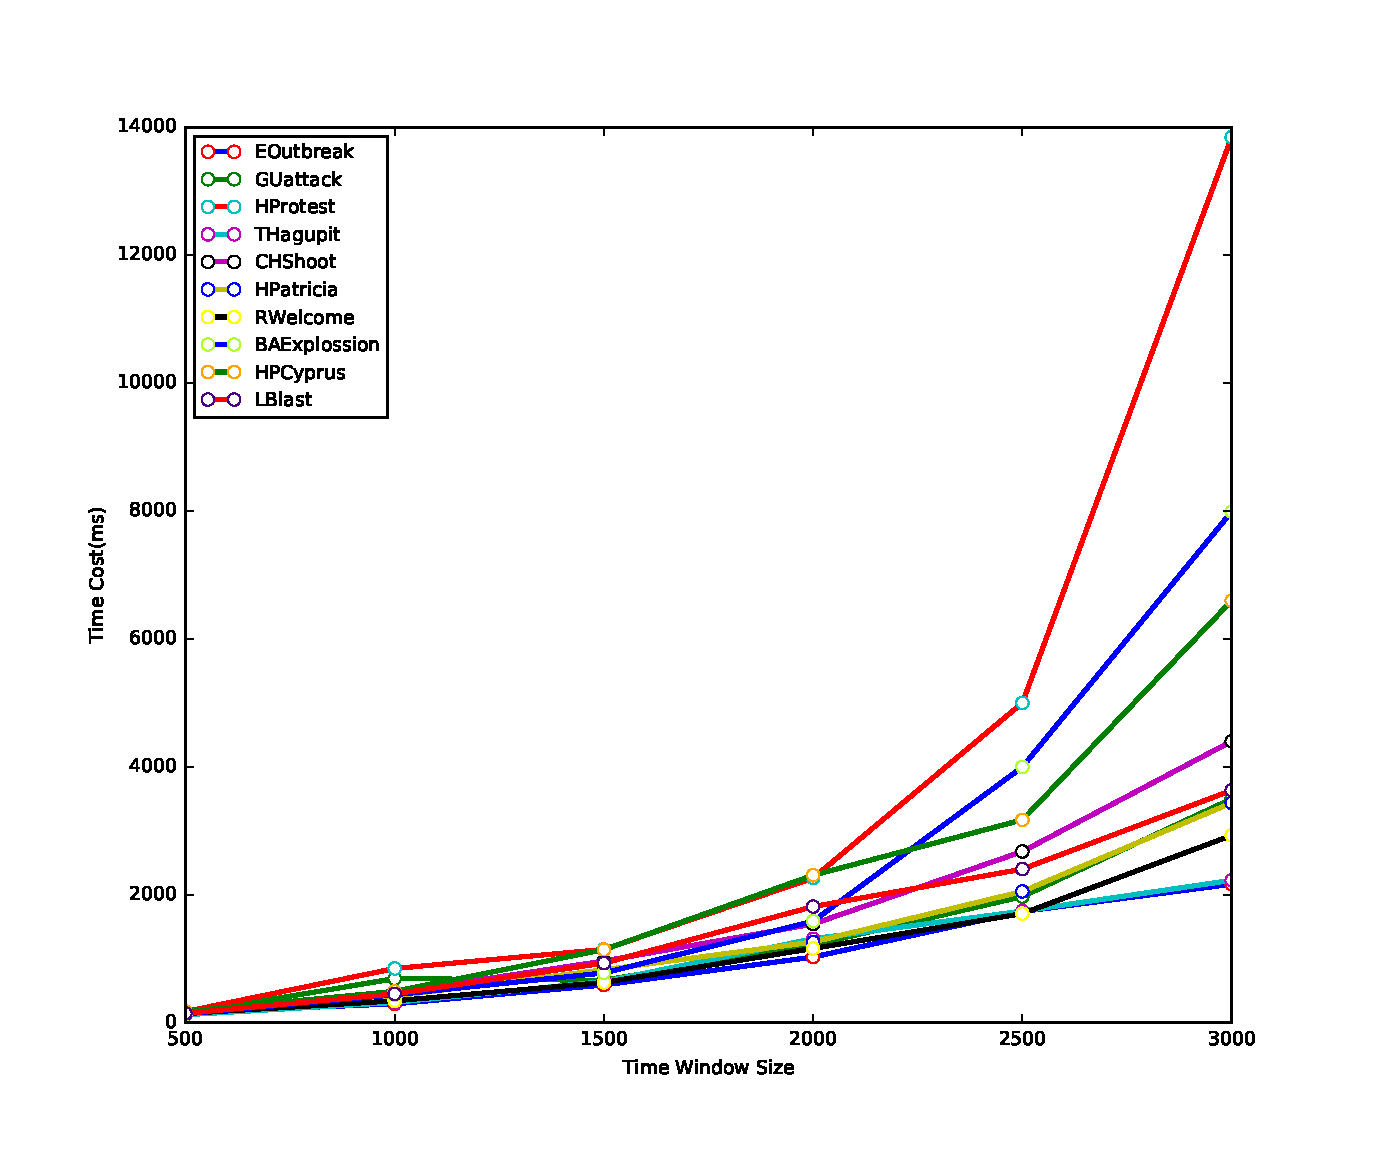
\includegraphics[scale=0.5]{window-timecost.eps}

\end{figure}

\section{Conclusion}\label{sec:conclusion}

\end{document}
